\chapter{Exchange rate data}\label{ch:exchangerate}

% Use of and challenge with exchange rate data
Under reporting regimes such as EMIR, MiFIR and SFTR counterparties can report monetary amounts in different currencies. This enables supervisors to analyse individual transactions very accurately, but for the purpose of calculating comparable market statistics, the reported values must be converted into a single -- usually the domestic -- currency. To this end, it is necessary to have a clean exchange rate data set, which can be easily merged with reporting data to perform the necessary transformations. To create this data set, we follow \parencite{ESMA.2018}, where publicly available exchange rates from the European Central Bank (ECB) are used as main data source. But since there are reports, where monetary amounts are reported in more exotic currencies not covered by the ECB data set, additional exchange rate data from other sources such as the Bank for International Settlements (BIS) or commercial data providers should be used to achieve greater coverage.

\begin{figure}[h!]
	\centering
	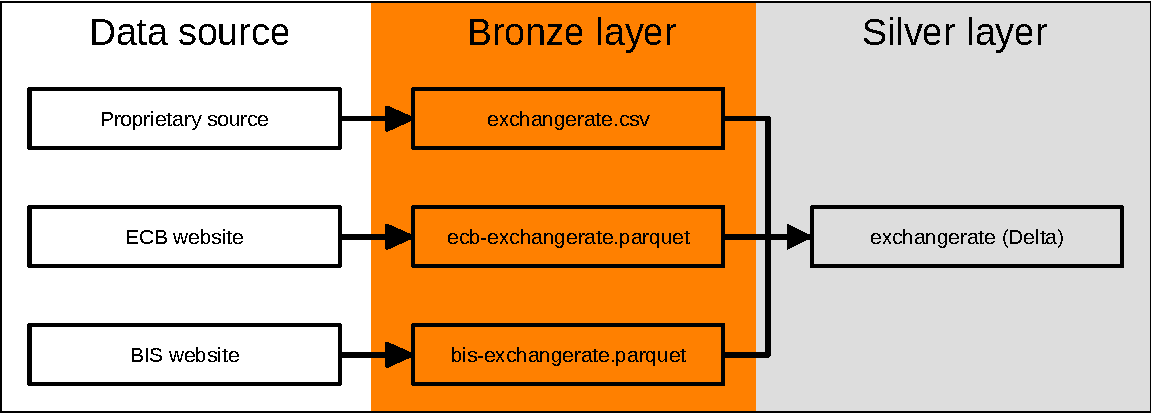
\includegraphics[height=5cm]{exchangerate-architecture}
	\caption{Data pipeline of exchange rate data.}
	\label{fig:function_exchangerate}
\end{figure}

Figure \ref{fig:function_exchangerate} illustrates the data pipeline used to generate a clean exchange rate data set. The pipeline consists of the following parts:
%
\begin{itemize}
	\item Download exchange rate data from the ECB's website and store the result in the bronze layer. As suggested in \textcite{Strengholt.2025}, the structure of the data is preserved. However, the downloaded Zip-file is unzipped and the content of the enclosed csv-file is converted into the Parquet file format. The archive itself is fetched and unpacked in a temporary directory on the local disk of the driver, so that only the resulting Parquet file ever reaches the data lake. This matters in a cloud deployment, where the Bronze layer is an object store volume that should not be burdened with files that are deleted again moments later.
	\item Optional: Download exchange rate data from the BIS's website and store the result in the bronze layer, following the same procedure as for the ECB data. Note that the BIS quotes its bulk exchange rate statistics against the US dollar and reports average rather than reference rates. The pipeline therefore converts these quotes into euro terms using the ECB's EUR/USD reference rate of the same day before the sources are combined, and drops the days for which the ECB does not provide such a rate.
	\item Optional: Download exchange rate data from a commercial data provider and transform it into the structure described in the annex document \emph{Annex - Exchange Rates - Data Dictionary.xlsx}. Save the result as the CSV file \verb|exchangerate.csv| in the Bronze layer as specified in the directory tree in figure \ref{fig:dirstruct_exchangerate}. The CSV file format was chosen, because it allows to impose a schema, which allows for better data validation and contributes to more stability. The schema is declared in the module, since this is the one source whose shape the pipeline does not learn from the file a publisher sent, and the columns of the file therefore have to be the ones of the annex document and in its order. Nothing in the module writes into that folder; the file is placed there by whoever maintains the quotes, as in the entity master data and the market price data modules.

	The file is checked before it is combined, and refused as a whole where a row would be misread: a reference date not written as \verb|YYYY-MM-DD|, a base currency other than the euro, a rate that is missing or not positive, or one day and currency pair quoted twice. The first of these matters most. The combination compares reference dates as text -- to find the date every source reaches, to cut the sources back to it, and to decide which source wins a day -- so a date written differently from the ECB's is not the same day to it. Without the check, a single row dated \verb|2020-10-5| beside ECB rates reaching 31 December would cut the whole table, every currency, back to 6 October, because \verb|2020-10-5| sorts before \verb|2020-10-06| as text, and leave two days with two rates each.
	\item Combine the data sets in the Bronze layer. Only use data up to the latest date in the data set in the least up-to-date sample. This should ensure that the exchange rate data set is always complete.
	\item Clean the data to avoid duplicated values. Where more than one source quotes the same currency pair on the same day, the \emph{fincommons} Python package prefers proprietary data over ECB data over BIS data, and only the winning quote is carried forward. The precedence is expressed as an explicit rank of the sources rather than as an ordering of the combined table, because the order in which the rows of a union arrive is not guaranteed and a rule that relies on it would silently change with the query plan.
	\item Fill the days on which no source quotes -- weekends, holidays and the gaps a source leaves behind -- with the last rate quoted on or before that day, so that the resulting data set holds one row per calendar day and currency pair. The fill follows the time series of the currency pair rather than that of an individual source, since the quote that closes a gap need not come from the source that opened it. Filling each source separately would leave a hole wherever the sources alternate, and an amount dated in such a hole would convert to nothing. The fill stops at the last quote of a pair rather than running on to the cutoff date, and days before the first quote of a pair are not filled either: a currency that ceases to be quoted ends with its last observation instead of carrying a stale rate forward indefinitely.

	Which rows are filled is recorded in the column \verb|IMPUTED|, which is true on a day whose rate was carried from an earlier quote and false on a day a source quoted. Wherever the ECB is the source, the imputed days are the weekends and the TARGET closing days, on which it does not publish; any other day without a quote is marked as well, whatever the reason for the gap, since a carried rate is imputed either way. A quote a source makes on a weekend is not imputed, and a re-based cross rate is imputed where either of the two euro rates it is computed from is. The column lets an analysis restrict itself to quoted rates, or see how much of a result rests on carried ones.
	\item Where an organisation does not have the euro as its national currency, data engineers can re-base the data so that the resulting data set contains exchange rates that correspond to the domestic currency. This is achieved via the transformation
	$$P^{other/domestic}_t = \frac{P^{other/EUR}_t}{P^{domestic/EUR}_t}.$$
	The transformation is applied to the combined data set, so that quotes originating from the proprietary source and the BIS are re-based along with those of the ECB. The euro is added as a quoted currency against the new base, while the new base currency is not quoted against itself.
	\item Store the result in directory \verb|exchangerate| in the Silver layer. The structure and content of the resulting data set are described in the annex document \emph{Annex - Exchange Rates - Data Dictionary.xlsx}. Each run recomputes the table in full rather than adding to it.
\end{itemize}

The table is written as Parquet or as Delta, which the update functions take as an argument. Parquet is the default, because it is the format every engine reads without a further dependency, which is what a table meant to be shared should be. Delta is worth asking for where the table may be queried while it is rebuilt: a Delta update replaces it in a single transaction, so that a reader sees either the previous version in full or the new one and never a half-written file, and the previous versions remain readable. A Parquet update deletes the table before it writes the new one, which leaves a window in which a reader finds it missing. The table is read back in whichever of the two formats it is stored in, so the choice does not have to be repeated when it is queried, and switching an existing table from Parquet to Delta means deleting the directory first, since Delta will not adopt Parquet files it has no transaction log for.

Figure \ref{fig:dirstruct_exchangerate} shows the directory structure that is used for the implementation of this pipeline.

% Directory tree
\begin{figure}[h!]
	\centering
	\begin{subfigure}[t]{.48\textwidth}
		\centering
		\begin{forest}
			for tree={
				%font=\ttfamily,
				grow'=0,
				child anchor=west,
				parent anchor=south,
				anchor=west,
				calign=first,
				edge path={
					\noexpand\path [draw, \forestoption{edge}]
					(!u.south west) +(7.5pt,0) |- node[fill,inner sep=1.25pt] {} (.child anchor)\forestoption{edge label};
				},
				before typesetting nodes={
					if n=1
					{insert before={[,phantom]}}
					{}
				},
				fit=band,
				before computing xy={l=15pt},
			}
			[bronze
			[exchangerate
			[ecb
			[ecb-exchangerate.parquet]
			]
			[bis
			[bis-exchangerate.parquet]
			]
			[internal
			[exchangerate.csv]
			]
			]
			]
		\end{forest}
		\caption{Bronze layer.}
	\end{subfigure} %
	~
	\begin{subfigure}[t]{.48\textwidth}
		\centering
		\begin{forest}
			for tree={
				%font=\ttfamily,
				grow'=0,
				child anchor=west,
				parent anchor=south,
				anchor=west,
				calign=first,
				edge path={
					\noexpand\path [draw, \forestoption{edge}]
					(!u.south west) +(7.5pt,0) |- node[fill,inner sep=1.25pt] {} (.child anchor)\forestoption{edge label};
				},
				before typesetting nodes={
					if n=1
					{insert before={[,phantom]}}
					{}
				},
				fit=band,
				before computing xy={l=15pt},
			}
			[silver
			[exchangerate
			[exchangerate]
			]
			[...]
			]
		\end{forest}
		\caption{Silver layer.}
	\end{subfigure}
	\caption{Directory structures for exchange rate data. In the Silver layer, \emph{exchangerate} is the directory of a table and not a single file.\label{fig:dirstruct_exchangerate}}
\end{figure}

Module \emph{exchangerate} of the \emph{fincommons} Python package contains the functions to perform the data processing steps described above. It is organised along the layers of the pipeline: one part declares the layout of the data lake and the schema of the proprietary source, a second downloads the public reference rates into the Bronze layer, and a third combines them into the Silver layer. The Silver layer part also provides the function \verb|convert2ccy|, with which data scientists convert a column of monetary amounts into a target currency. It is the reason why the Silver table is kept at a calendar-day grain: an amount agreed on a weekend still has to be converted, and a table that only held the quoted business days would leave such amounts unconverted. Amounts whose currency is already the target currency pass through at a rate of one, while amounts in a currency that the data set does not cover on the given date receive neither a rate nor a converted value, so that the absence of a quote remains visible instead of being silently approximated. The conversion itself runs on Spark, but the function accepts a Spark, pandas or polars data frame and returns the same kind of frame it was given, so a data scientist working on a sample in pandas does not have to move it into Spark first. Amounts are matched to rates by calendar day, so an amount dated with a time of day is converted at the rate of its day.

A run of the pipeline consists of the two downloads, of which the BIS one is optional, and the Silver layer update, which takes the target format, whether the BIS quotes are to be used and the currency to re-base to. The function \verb|update_exchangerate| runs all of them in one call and passes those arguments on. While it combines the sources it reports the last date each of them reaches together with the cutoff taken from them, because which source is holding the table back is the question a reader of the log asks. Further documentation on the module's functionality can be found in its README file.
